\documentclass[tikz,border=10pt]{standalone}
% Scale s = 0.015066 cm/px, origin at ink-bbox centre (302.5, 222.5)
\begin{document}
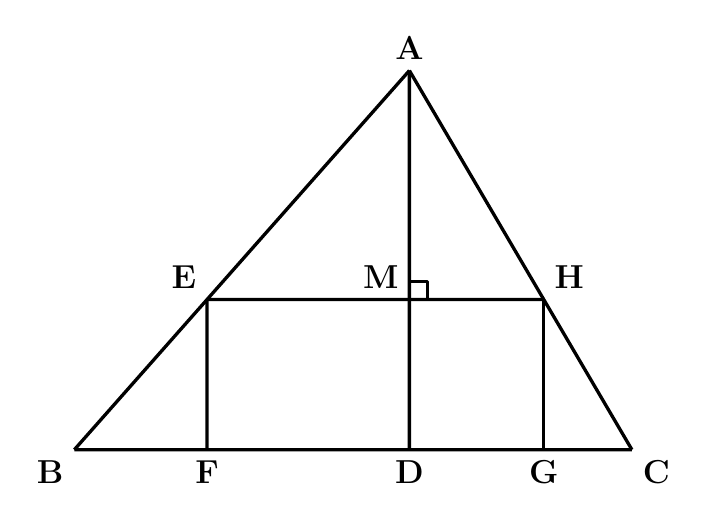
\begin{tikzpicture}[line width=1.2pt, line join=round, font=\fontsize{12}{14.4}\selectfont]
  % Named coordinates (converted from pixels)
  \coordinate (A) at (0.7163241242403742,2.439838989353213);
  \coordinate (B) at (-3.5387984571863766,-2.3752490552544665);
  \coordinate (C) at (3.542356636627046,-2.375280259927158);
  \coordinate (D) at (0.7163029054096128,-2.375267806297697);
  \coordinate (E) at (-1.8532271198271963,-0.46785996374439);
  \coordinate (F) at (-1.8532355251909098,-2.3752564830595206);
  \coordinate (G) at (2.4228788598952056,-2.3752753267012725);
  \coordinate (H) at (2.422887265258919,-0.46787880738614185);
  \coordinate (M) at (0.7163113107733268,-0.46787128698256675);

  % Solid black segments (geometry unchanged)
  \draw (A) -- (B);
  \draw (B) -- (C);
  \draw (C) -- (A);
  \draw (A) -- (D);
  \draw (E) -- (H);
  \draw (E) -- (F);
  \draw (H) -- (G);

  % Right-angle mark at M (between MA up and MH right)
  \draw (M)++(0,0.229) -- ++(0.229,0) -- ++(0,-0.229);

  % Labels: upright bold serif, correct bindings (C at bottom-right, H at (463,254), A only at apex)
  \node[above] at (A) {\textbf{A}};
  \node[below left] at (B) {\textbf{B}};
  \node[below right] at (C) {\textbf{C}};
  \node[below] at (D) {\textbf{D}};
  \node[above left] at (E) {\textbf{E}};
  \node[below] at (F) {\textbf{F}};
  \node[below] at (G) {\textbf{G}};
  \node[above right] at (H) {\textbf{H}};
  \node[above left] at (M) {\textbf{M}};
\end{tikzpicture}
\end{document}
% GEOAGENT_REPAIR_V1 c18a466396f54661 89858f3dffb8db1adcad5100b9c173c3e81ac7ac2c0cd5ad6c9edc524f8fafd3